\chapter{Ergebnisse} % (fold)
\label{sec:ergebnisse}
Im Nachfolgenden werden die Ergebnisse der Latenztests der oben eingeführten APIs dargestellt. Die konkreten Zahlen, auf denen die Grafiken beruhen sind im Kapitel Appendix zu finden.

\noindent
Zunächst wurde, wie in Abbildung 7.1 zu sehen, mittels HEAD Request ermittelt, ob die API verfügbar ist und welche Latenz zwischen Client und Server entsteht, ohne eine Datenabfrage auszuführen. Hierbei kann man beobachten, dass die Latenz von PostGraph und Neo4Graph sehr dicht beieinander liegen. REST basierte APIs hatten in diesem Experiment eine Latenz die deutlich variierte.

\noindent
Daraufhin wurden die Latenzen des parametrisierten API-Endpunktes ermittelt. In den Abbildungen 7.2 bis 7.5 wurden diese Ergebnisse in einem Koordinatensystem dargestellt. Die x-Achse repräsentiert die Menge der Tupel, welche angefordert wurden. Aufgrund der hohen Menge der Ergebnistupel wurde diese Achse logarithmisch dargestellt. Auf der z-Achse ist die Latenz in Millisekunden zu sehen. Die verschiedenen Graphen innerhalb der Abbildungen beschreiben die Menge der Joins, bei relationalen Datenbanken, oder Kanten, bei Graphdatenbanken. Rot (Kreis) steht hierbei für null, Blau (Quadrat) steht für eins und Orange (Diamant) steht hierbei für zwei. 
\newline
Bei PostREST (vgl. Abb. 7.2) steigt somit die Latenz mit der Menge der Ergebnistupeln exponentiell an. Zudem ist zu erkennen, dass bei einer Menge von 100.000 Ergebnistupeln die Menge der Joins deutlich Einfluss auf die Latenz nehmen. Hierbei ist eine Anfrage die weniger Joins verwendet (Rot) mit 426,5 Millisekunden deutlich performanter, als eine Abfrage die mehrere Joins (Orange) verwendet, welche 492,5 Millisekunden benötigt. Bei niedrigerer Tupelzahl wirken sich Joins nicht, bzw. nur in sehr geringen Maß auf die Latenz der Anfrage aus.
\newline
PostGraph zeigt in Abbildung 7.3 ein ähnliches Bild, jedoch mit einer deutlich höheren Latenz bei einer Anfragengröße von 100.000 Tupel. Die GraphQL API ist hier mit 1831 Millisekunden um einen Faktor von 3,7 langsamer als die REST API, welche auf derselben Datenbank basiert.
\newline
Bei Verwendung einer Neo4j Datenbank in Kombination mit einer REST-API (vgl. Abb. 7.4) fällt auf, dass die Anfragen mit geringer Tupelzahl eine sehr ähnliche Latenz aufweisen. Bei höherer Tupelzahl liegt die Anfragedauer jedoch deutlich höher als mit einer relationalen Datenbank. Hierbei erkennt man jedoch, dass Anfragen, welche mehrere Kanten nutzen schneller bearbeitet werden können. So benötigt eine Anfrage, welche ohne das Nutzen einer Kante auskommt, 1673 Millisekunden. Wenn man nun die Komplexität erhöht und für die Anfrage zwei Kanten verwendet, benötigt diese lediglich 1371 Millisekunden.
 \newline
Behält man nun die Datenbasis bei und nutzt eine GraphQL API (vgl. Abb. 7.5) fällt auf, dass erneut die Anfragedauer bei hoher Tupelzahl deutlich über der einer REST-API liegt. Ebenfalls ist hier zu beobachten, dass komplexere Anfragen schneller bearbeitet werden als weniger komplexe.
\newline
\noindent
Wie in Abbildung 7.6 zu sehen ist, hat die PostgreSQL REST-API eine höhere Latenzzeit als die GraphQL PostgeSQL. Dies deutet darauf hin, dass die GraphQL API bei der Abfrage eines spezifischen \texttt{Person} Objekts, anhand der \texttt{Person}-ID in Kombination mit einer relationalen Datenbank effizientere Abfragen und eine bessere Performance bei der Verarbeitung bietet. Ähnliches zeigt sich bei einer Neo4j Datenbank. Auch hier hat die Neo4j GraphQL API niedrigere Latenzzeiten als die REST-API. Allerdings sind die Latenzen bei Neo4j minimal höher als bei dem relationalen Pendant. Das deutet darauf hin, dass Postgres bei dieser Anfrage eine performantere Verarbeitung von Abfragen ermöglicht. Zusammenfassend kann man für diese Anfrage sagen, dass GraphQL sowohl in Kombination mit einer relationalen als auch einer Graphdatenbank eine niedrigere Latenz aufweist. Zudem ist Postgres bei dieser Anfrage insgesamt minimal performanter als Neo4j.
\newline
In Abbildung 7.7 sind die Latenzen für die komplexere Anfrage, die 5000 \texttt{Person} Objekte aus der Datenbank zurückliefert dargestellt. GraphQL hat hierbei sowohl bei der relationalen Datenbank als auch bei der Graphdatenbank im Median eine niedrigere Latenz. REST ist somit in beiden Fällen die weniger performantere API.
\newline
Wenn nun die Anfragekomplexität steigt, wodurch sich die Abhängigkeit zwischen den Objekten in der Datenbank erhöht, ist deutlich zu sehen, dass die Streuung bei der Postgres GraphQL API höher ist als bei allen anderen APIs (vgl. Abb.7.8). Der Median liegt jedoch deutlich niedriger. Die Neo4j REST-API liegt in diesem Fall deutlich über allen anderen APIs. Gefolgt von der PortgeSQL REST-API. Beide GraphQL APIs weißen erneut eine deutlich niedrigere Latenz auf.
\newline
Bei der Speicherung in eine Datenbank ist ein deutlich anderes Bild zu sehen. Wie in Abbildung 7.9 zusehen, ist hierbei die Postgres REST-API diejenige mit der geringsten Latenz. Dicht gefolgt von der Postgres GraphQL API. Eine deutlich höhere Latenz ist bei den Neo4j APIs zu erkennen. Hierbei ist allerdings die GraphQL API die performantere.


\begin{figure}[htbp]
 \centering
	\begin{tikzpicture}
	    \begin{axis}[
	        boxplot/draw direction=y, 
	        xlabel={API}, 
	        ylabel={ms}, 
	        xtick={1,2,3,4}, 
	        xticklabels={Post Rest, Post Graph, Neo4 Rest, Neo4 Graph}, 
	        ymin=50, ymax=65,
	       ytick distance=1,
                  width=15cm,
	       height= 18cm
	    ]
	       \addplot+[
	            boxplot prepared={
	                median=52,
	                upper quartile=55,
	                lower quartile=52, 
	                upper whisker=59,
	                lower whisker=51
	            },
	            draw=black
	        ] coordinates {};
	        \addplot+[
	            boxplot prepared={
	                median=53,
	                upper quartile=53,
	                lower quartile=53, 
	                upper whisker=54,
	                lower whisker=52
	            },
	            draw=black
	        ] coordinates {};
	         \addplot+[
	            boxplot prepared={
	                median=52,
	                upper quartile=58,
	                lower quartile=52, 
	                upper whisker=63,
	                lower whisker=51
	            },
	            draw=black
	        ] coordinates {};
	       \addplot+[
	            boxplot prepared={
	                median=52,
	                upper quartile=53,
	                lower quartile=52, 
	                upper whisker=54,
	                lower whisker=51
	            },
	            draw=black
	        ] coordinates {};
	    \end{axis}
	\end{tikzpicture}
\caption{HEAD /api/resource}
\end{figure}




\begin{figure}
\centering
\begin{tikzpicture}[scale=1.9]
\begin{axis}[
    axis lines = middle,
    xlabel = {x},
    ylabel = {y},
    zlabel = {z},
    xmode = log,
    width=10cm,
    height=10cm,
    grid = major,
    enlarge x limits = true,
    view={0}{0},
    ymin=0, ymax=3,  
]
% Linie und Punkte für die ersten Punkte (rot)
\addplot3+[
    only marks, 
    mark=*,
    red,
    mark options={fill=red} % Innere des Punktes rot färben
] coordinates {
    (1, 0, 111)
    (100, 0, 121)
    (1000, 0, 135)
    (10000, 0, 272)
    (100000, 0, 426.5)
};
\addplot3[
    red, % Linie durch die Punkte
    mark=none % keine Markierungen an der Linie
] coordinates {
    (1, 0, 111)
    (100, 0, 121)
    (1000, 0, 135)
    (10000, 0, 272)
    (100000, 0, 426.5)
};
% Linie und Punkte für die zweiten Punkte (blau)
\addplot3+[
    only marks, 
    mark=square*,
    blue,
    mark options={fill=blue} % Innere des Punktes blau färben
] coordinates {
    (1, 1, 111)
    (100, 1, 122)
    (1000, 1, 134)
    (10000, 1, 271.5)
    (100000, 1, 468)
};
\addplot3[
    blue, % Linie durch die Punkte
    mark=none % keine Markierungen an der Linie
] coordinates {
    (1, 1, 111)
    (100, 1, 122)
    (1000, 1, 134)
    (10000, 1, 271.5)
    (100000, 1, 468)
};
% Linie und Punkte für die vierten Punkte (orange)
\addplot3+[
    only marks, 
    mark=diamond*,
    orange,
    mark options={fill=orange} % Innere des Punktes orange färben
] coordinates {
    (1, 3, 111)
    (100, 3, 119.5)
    (1000, 3, 146)
    (10000, 3, 267)
    (100000, 3, 492.5)
};
\addplot3[
    orange, % Linie durch die Punkte
    mark=none % keine Markierungen an der Linie
] coordinates {
    (1, 3, 111)
    (100, 3, 119.5)
    (1000, 3, 146)
    (10000, 3, 267)
    (100000, 3, 492.5)
};
\end{axis}
\end{tikzpicture}
\caption{PostREST parametriesierte Abfragen}
\end{figure}

\begin{figure}
\centering
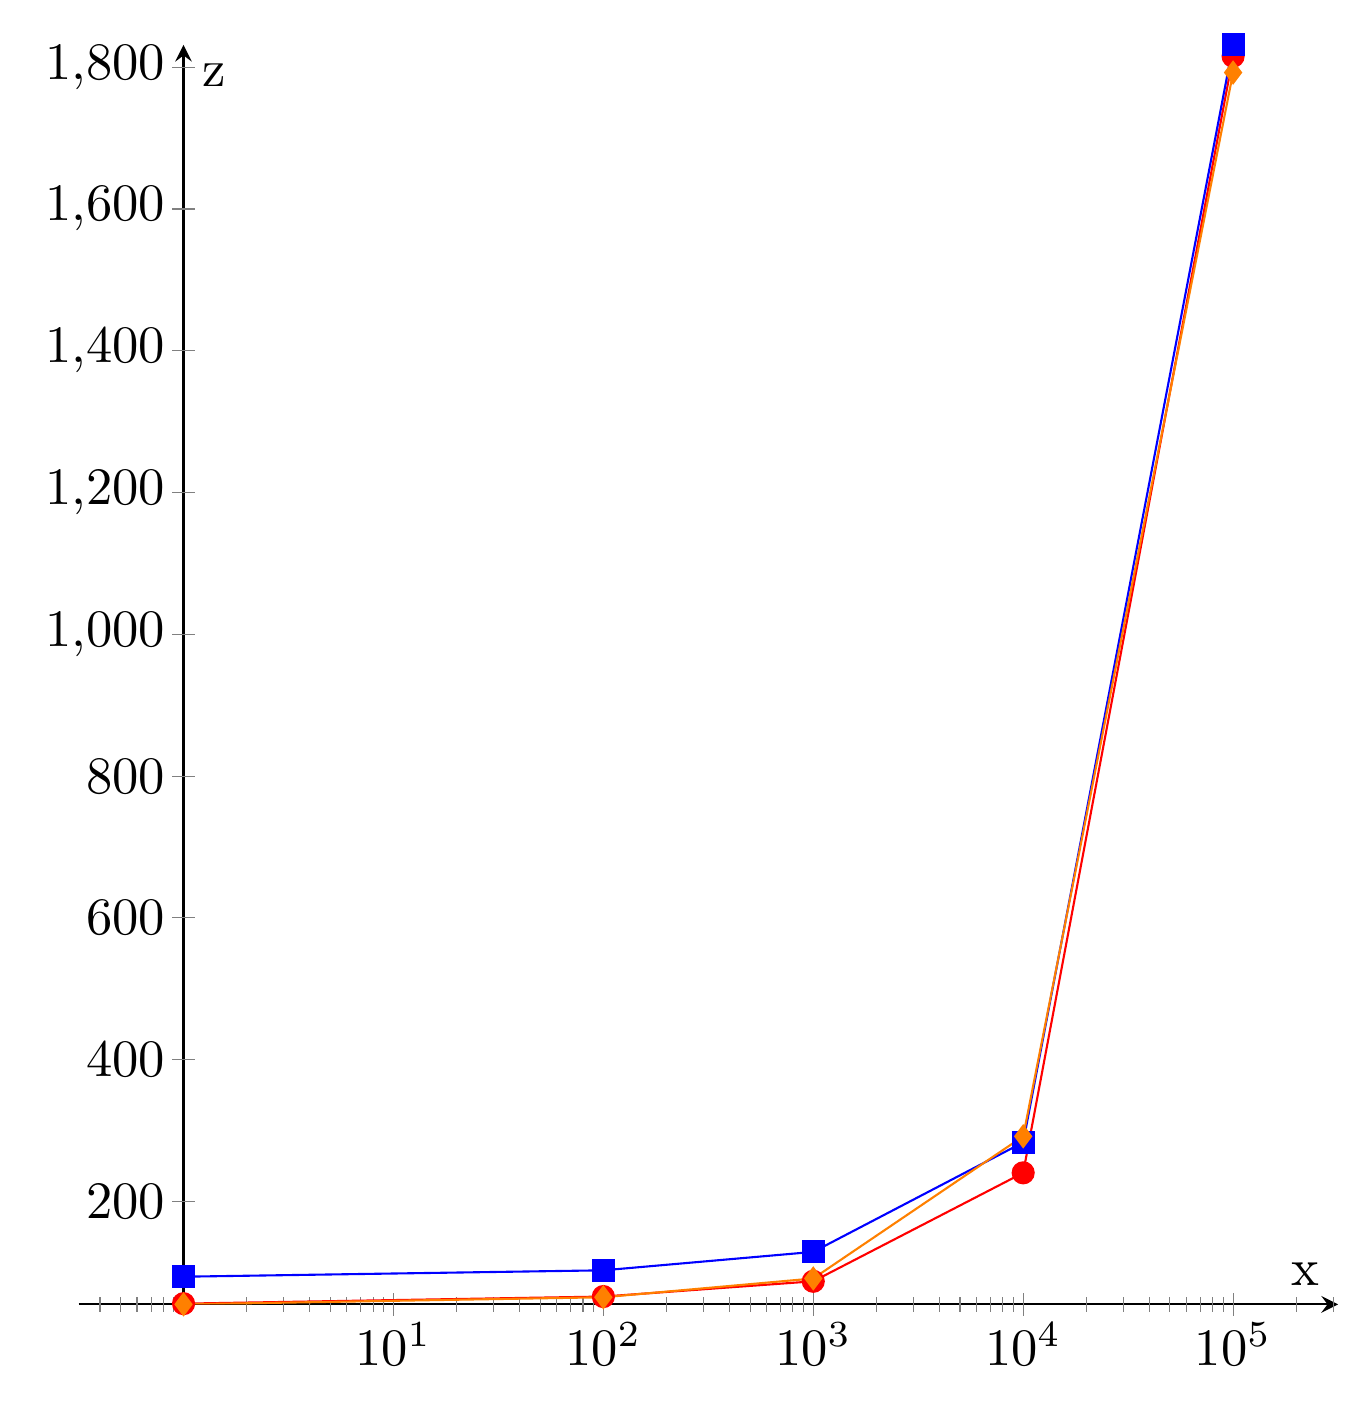
\begin{tikzpicture}[scale=1.9]
\begin{axis}[
    axis lines = middle,
    xlabel = {x},
    ylabel = {y},
    zlabel = {z},
    xmode = log,
    width=10cm,
    height=10cm,
    grid = major,
    enlarge x limits = true,
    view={0}{0},
    ymin=0, ymax=3,  
]
% Linie und Punkte für die ersten Punkte (rot)
\addplot3+[
    only marks, 
    mark=*,
    red,
    mark options={fill=red} % Innere des Punktes rot färben
] coordinates {
    (1, 0, 56)
    (100, 0, 66)
    (1000, 0, 87.5)
    (10000, 0, 240.5)
    (100000, 0, 1815.5)
};
\addplot3[
    red, % Linie durch die Punkte
    mark=none % keine Markierungen an der Linie
] coordinates {
    (1, 0, 56)
    (100, 0, 66)
    (1000, 0, 87.5)
    (10000, 0, 240.5)
    (100000, 0, 1815.5)
};
% Linie und Punkte für die zweiten Punkte (blau)
\addplot3+[
    only marks, 
    mark=square*,
    blue,
    mark options={fill=blue} % Innere des Punktes blau färben
] coordinates {
    (1, 1, 94)
    (100, 1, 103)
    (1000, 1, 129)
    (10000, 1, 283.5)
    (100000, 1, 1831.5)
};
\addplot3[
    blue, % Linie durch die Punkte
    mark=none % keine Markierungen an der Linie
] coordinates {
    (1, 1, 94)
    (100, 1, 103)
    (1000, 1, 129)
    (10000, 1, 283.5)
    (100000, 1, 1831.5)
};
% Linie und Punkte für die vierten Punkte (orange)
\addplot3+[
    only marks, 
    mark=diamond*,
    orange,
    mark options={fill=orange} % Innere des Punktes orange färben
] coordinates {
    (1, 3, 55)
    (100, 3, 65)
    (1000, 3, 91.5)
    (10000, 3, 292)
    (100000, 3, 1792.5)
};
\addplot3[
    orange, % Linie durch die Punkte
    mark=none % keine Markierungen an der Linie
] coordinates {
    (1, 3, 55)
    (100, 3, 65)
    (1000, 3, 91.5)
    (10000, 3, 292)
    (100000, 3, 1792.5)
};
\end{axis}
\end{tikzpicture}
\caption{PostGraph parametriesierte Abfragen}
\end{figure}



\begin{figure}
\centering
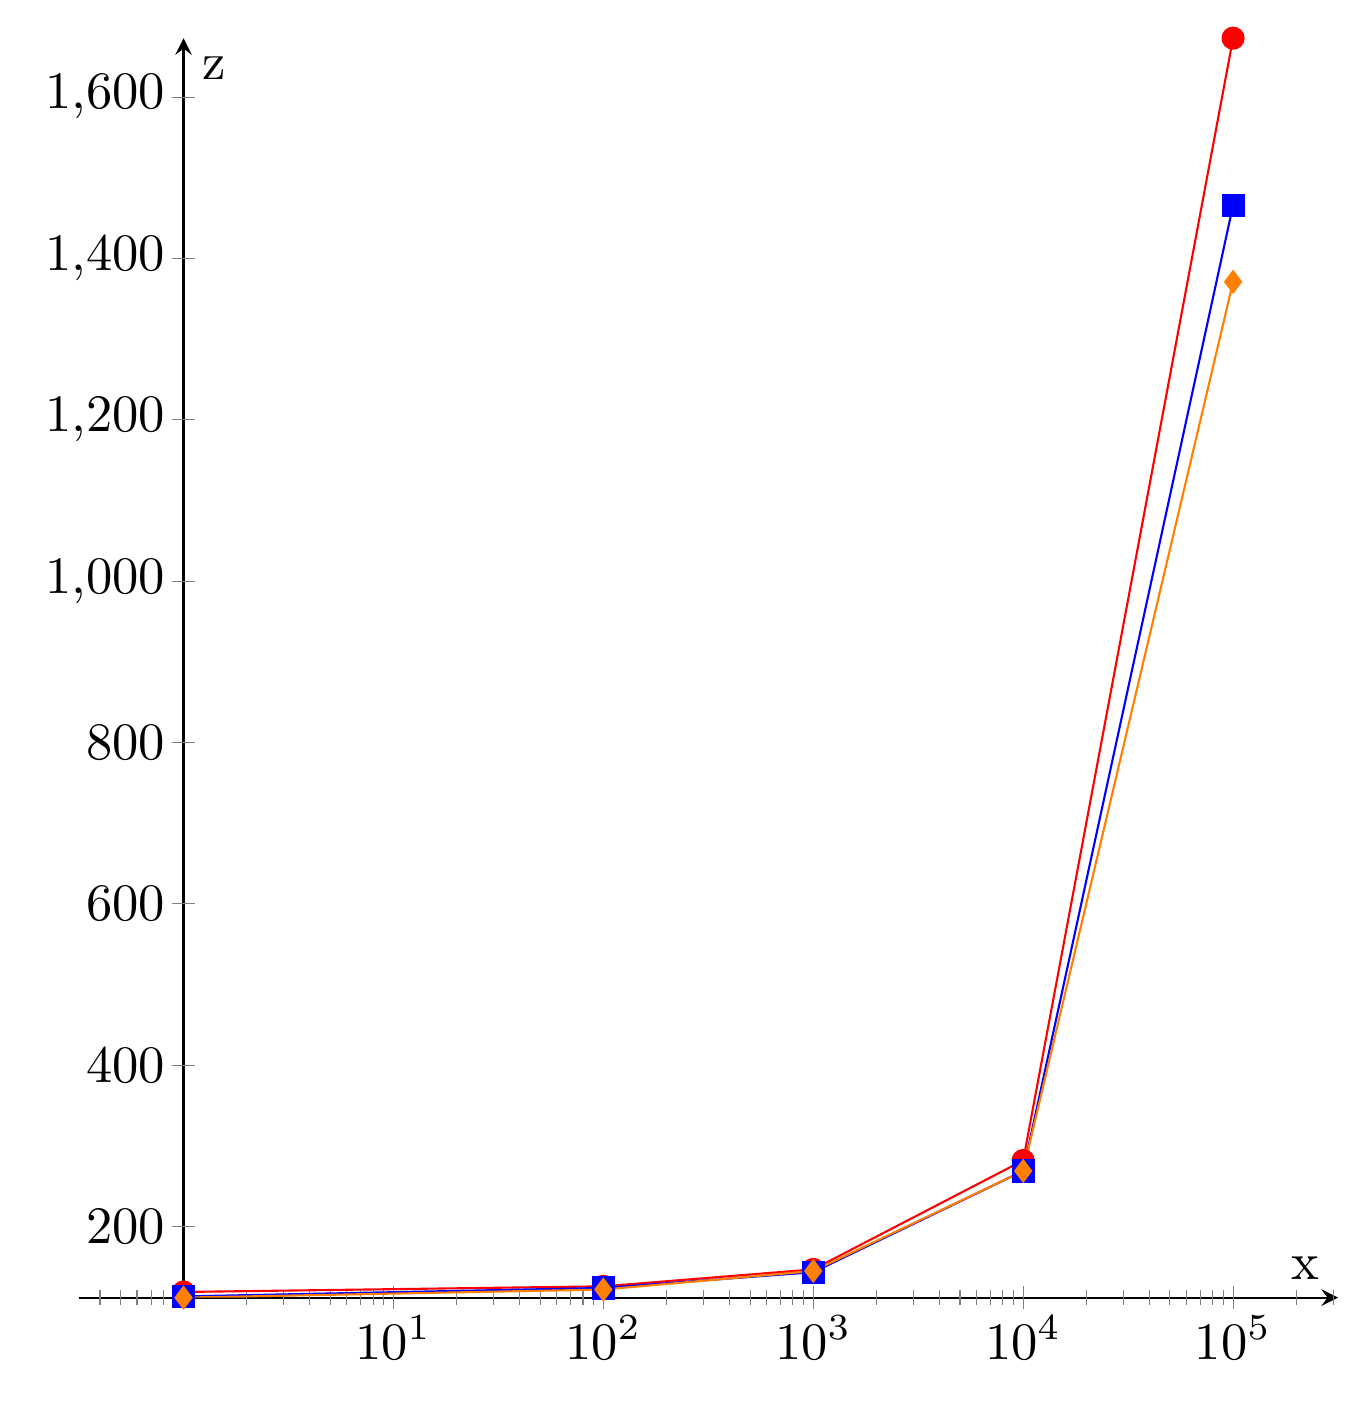
\begin{tikzpicture}[scale=1.9]
\begin{axis}[
    axis lines = middle,
    xlabel = {x},
    ylabel = {y},
    zlabel = {z},
    xmode = log,
    width=10cm,
    height=10cm,
    grid = major,
    enlarge x limits = true,
    view={0}{0},
    ymin=0, ymax=3,  
]
% Linie und Punkte für die ersten Punkte (rot)
\addplot3+[
    only marks, 
    mark=*,
    red,
    mark options={fill=red} % Innere des Punktes rot färben
] coordinates {
    (1, 0, 119)
    (100, 0, 126)
    (1000, 0, 147)
    (10000, 0, 282)
    (100000, 0, 1673)
};
\addplot3[
    red, % Linie durch die Punkte
    mark=none % keine Markierungen an der Linie
] coordinates {
    (1, 0, 119)
    (100, 0, 126)
    (1000, 0, 147)
    (10000, 0, 282)
    (100000, 0,1673)
};
% Linie und Punkte für die zweiten Punkte (blau)
\addplot3+[
    only marks, 
    mark=square*,
    blue,
    mark options={fill=blue} % Innere des Punktes blau färben
] coordinates {
    (1, 1, 113.5)
    (100, 1, 124)
    (1000, 1, 143.5)
    (10000, 1, 269)
    (100000, 1, 1466)
};
\addplot3[
    blue, % Linie durch die Punkte
    mark=none % keine Markierungen an der Linie
] coordinates {
    (1, 1, 113.5)
    (100, 1, 124)
    (1000, 1, 143.5)
    (10000, 1, 269)
    (100000, 1, 1466)
};
% Linie und Punkte für die vierten Punkte (orange)
\addplot3+[
    only marks, 
    mark=diamond*,
    orange,
    mark options={fill=orange} % Innere des Punktes orange färben
] coordinates {
    (1, 3, 112)
    (100, 3, 122)
    (1000, 3, 145)
    (10000, 3, 269)
    (100000, 3, 1371)
};
\addplot3[
    orange, % Linie durch die Punkte
    mark=none % keine Markierungen an der Linie
] coordinates {
    (1, 3, 112)
    (100, 3, 122)
    (1000, 3, 145)
    (10000, 3, 269)
    (100000, 3, 1371)
};
\end{axis}
\end{tikzpicture}
\caption{Neo4REST parametriesierte Abfragen}
\end{figure}


\begin{figure}
\centering
\begin{tikzpicture}[scale=1.9]
\begin{axis}[
    axis lines = middle,
    xlabel = {x},
    ylabel = {y},
    zlabel = {z},
    xmode = log,
    width=10cm,
    height=10cm,
    grid = major,
    enlarge x limits = true,
    view={0}{0},
    ymin=0, ymax=3,  
]
% Linie und Punkte für die ersten Punkte (rot)
\addplot3+[
    only marks, 
    mark=*,
    red,
    mark options={fill=red} % Innere des Punktes rot färben
] coordinates {
    (1, 0, 58)
    (100, 0, 70)
    (1000, 0, 105.5)
    (10000, 0, 391)
    (100000, 0, 2726.5)
};
\addplot3[
    red, % Linie durch die Punkte
    mark=none % keine Markierungen an der Linie
] coordinates {
    (1, 0, 58)
    (100, 0, 70)
    (1000, 0, 105.5)
    (10000, 0, 391)
    (100000, 0,2726.5)
};
% Linie und Punkte für die zweiten Punkte (blau)
\addplot3+[
    only marks, 
    mark=square*,
    blue,
    mark options={fill=blue} % Innere des Punktes blau färben
] coordinates {
    (1, 1, 59)
    (100, 1, 70)
    (1000, 1, 102.5)
    (10000, 1, 330)
    (100000, 1, 2484.5)
};
\addplot3[
    blue, % Linie durch die Punkte
    mark=none % keine Markierungen an der Linie
] coordinates {
    (1, 1, 59)
    (100, 1, 70)
    (1000, 1, 102.5)
    (10000, 1, 330)
    (100000, 1, 2484.5)
};
% Linie und Punkte für die vierten Punkte (orange)
\addplot3+[
    only marks, 
    mark=diamond*,
    orange,
    mark options={fill=orange} % Innere des Punktes orange färben
] coordinates {
    (1, 3, 57)
    (100, 3, 69)
    (1000, 3, 96)
    (10000, 3, 317)
    (100000, 3, 2396.5)
};
\addplot3[
    orange, % Linie durch die Punkte
    mark=none % keine Markierungen an der Linie
] coordinates {
    (1, 3, 57)
    (100, 3, 69)
    (1000, 3, 96)
    (10000, 3, 317)
    (100000, 3, 2396.5)
};
\end{axis}
\end{tikzpicture}
\caption{Neo4Graph parametriesierte Abfragen}
\end{figure}



\begin{figure}[htbp]
 \centering
	\begin{tikzpicture}
	    \begin{axis}[
	        boxplot/draw direction=y, 
	        xlabel={API}, 
	        ylabel={ms}, 
	        ytick distance=5,
	        xtick={1,2,3,4}, 
	        xticklabels={Post Rest, Post Graph, Neo4 Rest, Neo4 Graph}, 
	        ymin=50, ymax=150,
		width=15cm,
		height= 18cm
	    ]
	        \addplot+[
	            boxplot prepared={
	                median=109,
	                upper quartile=110,
	                lower quartile=108, 
	                upper whisker=113,
	                lower whisker=106
	            },
	            draw=black
	        ] coordinates {};
	        \addplot+[
	            boxplot prepared={
	                median=56,
	                upper quartile=57,
	                lower quartile=55, 
	                upper whisker=60,
	                lower whisker=54
	            },
	            draw=black
	        ] coordinates {};
	        \addplot+[
	            boxplot prepared={
	                median=113,
	                upper quartile=114,
	                lower quartile=110, 
	                upper whisker=120,
	                lower whisker=108
	            },
	            draw=black
	        ] coordinates {};
	       \addplot+[
	            boxplot prepared={
	                median=59,
	                upper quartile=60,
	                lower quartile=58, 
	                upper whisker=63,
	                lower whisker=57
	            },
	            draw=black
	        ] coordinates {};
	    \end{axis}
	\end{tikzpicture}
\caption{GET /api/persons/:pid}
\end{figure}

\begin{figure}[htbp]
 \centering
	\begin{tikzpicture}
	    \begin{axis}[
	        boxplot/draw direction=y, 
	        xlabel={API}, 
	        ylabel={ms}, 
	        xtick={1,2,3,4}, 
	        xticklabels={Post Rest, Post Graph, Neo4 Rest, Neo4 Graph}, 
	        ymin=50, ymax=350,
                  ytick distance=20,
                  width=15cm,
	       height= 18cm
	    ]
	        \addplot+[
	            boxplot prepared={
	                median=268,
	                upper quartile=278,
	                lower quartile=265, 
	                upper whisker=297,
	                lower whisker=250
	            },
	            draw=black
	        ] coordinates {};
	        \addplot+[
	            boxplot prepared={
	                median=190,
	                upper quartile=197,
	                lower quartile=181, 
	                upper whisker=216,
	                lower whisker=165
	            },
	            draw=black
	        ] coordinates {};
	         \addplot+[
	            boxplot prepared={
	                median=266,
	                upper quartile=275,
	                lower quartile=259, 
	                upper whisker=291,
	                lower whisker=245
	            },
	            draw=black
	        ] coordinates {};
	       \addplot+[
	            boxplot prepared={
	                median=261,
	                upper quartile=267,
	                lower quartile=254, 
	                upper whisker=279,
	                lower whisker=241
	            },
	            draw=black
	        ] coordinates {};
	    \end{axis}
	\end{tikzpicture}
\caption{GET /api/persons}
\end{figure}

\begin{figure}[htbp]
 \centering
	\begin{tikzpicture}
	    \begin{axis}[
	        boxplot/draw direction=y, 
	        xlabel={API}, 
	        ylabel={ms}, 
	        xtick={1,2,3,4}, 
	        xticklabels={Post Rest, Post Graph, Neo4 Rest, Neo4 Graph}, 
	        ymin=50, ymax=220,
	        ytick distance=20,
                  width=15cm,
	       height= 18cm
	    ]
	        \addplot+[
	            boxplot prepared={
	                median=139,
	                upper quartile=142,
	                lower quartile=137, 
	                upper whisker=148,
	                lower whisker=135
	            },
	            draw=black
	        ] coordinates {};
	        \addplot+[
	            boxplot prepared={
	                median=88,
	                upper quartile=123,
	                lower quartile=85, 
	                upper whisker=180,
	                lower whisker=83
	            },
	            draw=black
	        ] coordinates {};
	         \addplot+[
	            boxplot prepared={
	                median=178,
	                upper quartile=184,
	                lower quartile=176, 
	                upper whisker=195,
	                lower whisker=173
	            },
	            draw=black
	        ] coordinates {};
	       \addplot+[
	            boxplot prepared={
	                median=59,
	                upper quartile=60,
	                lower quartile=58, 
	                upper whisker=62,
	                lower whisker=57
	            },
	            draw=black
	        ] coordinates {};
	    \end{axis}
	\end{tikzpicture}
\caption{GET /api/persons/:pid/projects/issues}
\end{figure}

\begin{figure}[htbp]
 \centering
	\begin{tikzpicture}
	    \begin{axis}[
	        boxplot/draw direction=y, 
	        xlabel={API}, 
	        ylabel={ms}, 
	        xtick={1,2,3,4}, 
	        xticklabels={Post Rest, Post Graph, Neo4 Rest, Neo4 Graph}, 
	        ymin=50, ymax=130,
	       ytick distance=5,
                  width=15cm,
	       height= 18cm
	    ]
	       \addplot+[
	            boxplot prepared={
	                median=56,
	                upper quartile=57,
	                lower quartile=55, 
	                upper whisker=60,
	                lower whisker=54
	            },
	            draw=black
	        ] coordinates {};
	        \addplot+[
	            boxplot prepared={
	                median=58,
	                upper quartile=60,
	                lower quartile=57, 
	                upper whisker=62,
	                lower whisker=55
	            },
	            draw=black
	        ] coordinates {};
	         \addplot+[
	            boxplot prepared={
	                median=89,
	                upper quartile=97,
	                lower quartile=83, 
	                upper whisker=118,
	                lower whisker=77
	            },
	            draw=black
	        ] coordinates {};
	       \addplot+[
	            boxplot prepared={
	                median=82,
	                upper quartile=87,
	                lower quartile=78, 
	                upper whisker=99,
	                lower whisker=73
	            },
	            draw=black
	        ] coordinates {};
	    \end{axis}
	\end{tikzpicture}
\caption{POST /api/persons/:pid/projects/:prid/issues}
\end{figure}

% chapter ergebnisse (end)